\documentclass[varwidth=true, border=2pt]{standalone}
\usepackage{tikz}

\begin{document}
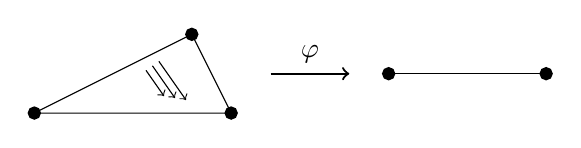
\begin{tikzpicture}
    \tikzstyle{point}=[circle,thick,draw=black,fill=black,inner sep=0pt,minimum width=4pt,minimum height=4pt]

    \node (a)[point] at (0,0) {};
    \node (b)[point] at (2.5,0) {};
    \node (c)[point] at (2,1) {};

    \begin{scope}[xshift=4.5cm, yshift=0.5cm]
        \node (d)[point] at (0,0) {};
        \node (e)[point] at (2,0) {};
    \end{scope}

    \begin{scope}[xshift=1.5cm,yshift=0.6cm,rotate=-55]
    \draw[->] (0,-0.1) -- (0.4,-0.1);
    \draw[->] (0, 0.0) -- (0.5, 0.0);
    \draw[->] (0, 0.1) -- (0.6, 0.1);
    \end{scope}

    \draw (a.center) -- (b.center) -- (c.center) -- cycle;
    \draw (d.center) -- (e.center);

    \draw[thick,->] (3,0.5) -- node[above] {$\varphi$} (4,0.5);
\end{tikzpicture}
\end{document}
